Um einen umfassenden theoretischen Hintergrund für das Experiment zu erhalten, werden hier unterschiedliche Themenbereiche erläutert. Zunächst geht es um die Magnetischen Momente von Atomen, dann denn um den Zeemann-Effekt und dann um das eigentliche optische Pumpen.
\subsection{Magnetische Momente von Atomen}
Eine rotierende elektrische Ladung erzeugt ein magnetisches Moment. Innerhalb eines Atoms trifft dies für verschiedene Rotationsbewegungen zu: Den Spin $\vec{S} $, den Bahndrehimpuls $\vec{L}$, den Gesamtdrehimpuls der Elektronenhülle $\vec{J}$, den Kernspin $\vec{I}$ und den Gesamtdrehimpuls des Atoms $\vec{F}$. Die Größen sind miteinander verknüpft:
\begin{align*}
	\vec{J} &= \vec{S} + \vec{L} \\
	\vec{F} &= \vec{J} + \vec{I}
\end{align*}
Die resultierenden magnetischen Momente $\vec{\mu}$ der Größen stehen jeweils antiparallel zu dem Drehvektor und sind proportional zum Betrag.
\begin{align*}
	\vec{\mu}_S &= - g_S \mu_B \vec{S} \\
	\vec{\mu}_L &= - \mu_B \vec{L} \\
	\vec{\mu}_J &= - g_J \mu_B \vec{J} \\
	\vec{\mu}_I &= -g_I \mu_K \vec{I} \\
	\vec{\mu}_F &= \vec{\mu}_J + \vec{\mu}_I
\end{align*}
 In den Proportionalitätsfaktor gehen das Bohrsche Magneton $\mu_B$ und das Kernmagneton $\mu_K$ sowie der Landé-Faktor $g$ ein, der für jedes Teilchen einen unterschiedlichen Wert annehmen kann. Die Beträge der magnetischen Momente entsprechen dem quantenmechanischen Erwartungswert und sind geometrisch mit Hilfe des Cosinus-Satzes (siehe Abb. \ref{fig:drehimpuls}) miteinander verknüpft.
 \begin{align}
 	| \vec{\mu}_S| &= g_S \mu_B \sqrt{S(S+1)} \notag\\
 	| \vec{\mu}_L| &=  \mu_B \sqrt{L(L+1)} \notag \\
 	| \vec{\mu}_J|  &= g_J \mu_B \sqrt{J(J+1)} = | \vec{\mu}_L | \cos{\beta} + |\vec{\mu}_S| \cos{\alpha} \notag \\
 	| \vec{\mu}_I| &= g_I \mu_K \sqrt{I(I+1)} \notag \\
 	|\vec{\mu}_F |&= g_F \vec{\mu} \sqrt{F(F+1)} = |\vec{\mu}_J| \cos(\vec{J}, \vec{F}) +|\vec{\mu}_I| \cos(\vec{I}, \vec{F}) \label{eq:mu_I}
 \end{align}
 Berücksichtigt man nun, dass, aufgrund der im Vergleich zum Elektron großen Masse des Kerns, $\mu_B >> \mu_K$ gilt, kann der letzte Term aus Gleichung \eqref{eq:mu_I} vernachlässigt werden und es folgt für den Landé-Faktor des gesamten Atoms
\begin{align}\label{eq:LandeF}
	g_F = \frac{g_J}{2}\frac{F(F+1) + J(J+1) - I(I+1)}{F(F+1)} \quad .
\end{align}

\begin{figure}
	\centering
	\subfigure{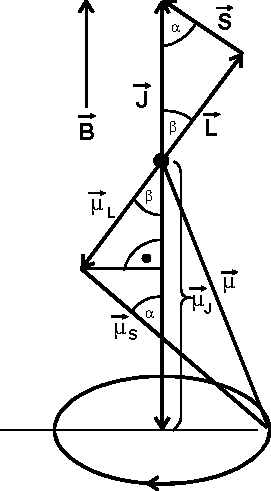
\includegraphics[width=0.25\textwidth]{Abb1.pdf}}
	\hspace{2cm}
	\subfigure{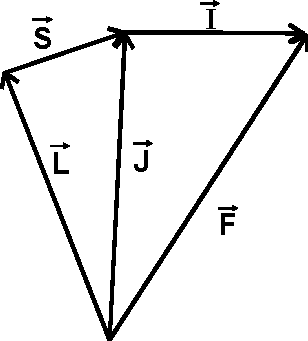
\includegraphics[width=0.25\textwidth]{Abb2.pdf}}\\
	\caption[Drehimpulse und magnetische Momente]{Geometrische Darstellung der Orientierungen des Drehimpulse und der magnetischen Momente \cite{\V}}
	\label{fig:drehimpuls}
\end{figure}

\clearpage 

\subsection{Zeemann-Effekt}
Ein magnetisches Moment $\vec{\mu}$ in einem äußeren Magnetfeld $\vec{B}$ hat eine potentielle Energie. Es sind nur parallel zu $\vec{B}$ stehende Anteile von $\vec{\mu}$ relevant. Ist das Magnetfeld in z-Richtung orientiert kann für $\vec{\mu}$ die Orientierungsquantenzahl $M_J$ eingesetzt werden. Sie ist quantisiert und läuft ganzzahlig von $-J$ bis $J$.
\begin{align}
	U_{\textrm{mag}} = - \vec{\mu} \cdot \vec{B} = M_J g_J \mu_B B
\end{align}
In einem Äußeren Magnetfeld spalten sich also die unterschiedlichen Energieniveaus auf. Das wird Zeemann-Effekt genannt. Wenn zusätzlich der Kernspin von null verschieden ist, spalten sich die Energieniveaus weiter auf. Man teilt die Aufspaltung in drei Bereiche ein: Die Feinstrukturaufspaltung durch den Eektronenspin, die Hyperfeinstrukturaufspaltung durch den Kernspin und die Zeemann-Aufspaltung durch das äußere Magnetfeld (siehe Abb.~\ref{fig:zeemann}). Die Energiedifferenz zwischen den einzelnen Niveaus ist dann
\begin{align}
\Delta U = g_F \mu_B B \quad .
\end{align}
Berücksichtigt man zusätzlich Spin-Bahn-Wechselwirkungen entstehen Terme, die quadratisch in B sind und bei starken Magnetfeldern ins Gewicht fallen. Die Formel ist als Breit-Rabi-Formel bekannt
\begin{align}
	\label{eq:quadrat}
	a = g_F \mu_B B +g_F^2 \mu_B^2 B^2 \frac{(1-2 M_F)}{\Delta E} - ... \quad .
\end{align}
Wobei $\Delta E$ die Energie der Hyperfeinaufspaltung zwischen den Niveaus mit den zugehörigen Quantenzahlen $F$ und $F+1$ ist.

\begin{figure}[H]
	\centering
	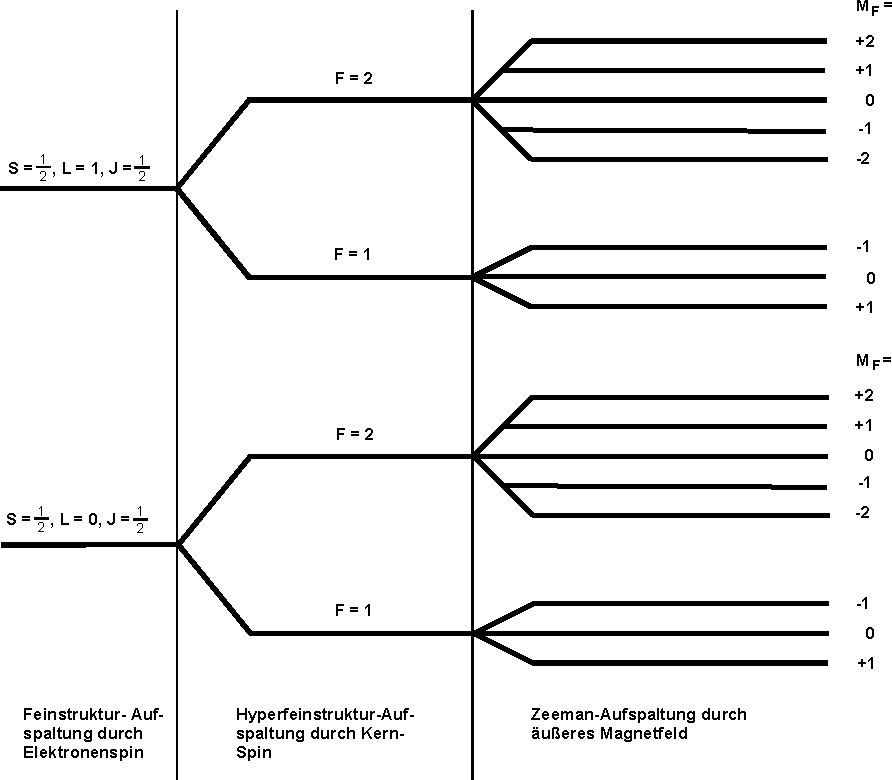
\includegraphics[width=0.8\textwidth]{Abb3.pdf}
	\caption[Zeemann-Effekt]{Aufspaltung der Energieniveaus in einem Magnetfeld \cite{\V}}
	\label{fig:zeemann}
\end{figure}


\subsection{Optisches Pumpen}
Im thermodynamischen Gleichgewicht ist bei zwei Niveaus unterschiedlicher Energie das  Niveau mit der niedrigeren Energie stärker besetzt. Für Laser ist es allerdings notwendig, dass das Niveau mit der höheren Energie stärker besetzt ist. Dieser Zustand wird als Besetzungsinversion bezeichnet. Das optische Pumpen ist eine Möglichkeit eine Besetzungsinversion zu erreichen. \\
Man benötigt hierzu ein System mit mindestens drei unterschiedlichen Energieniveaus. In diesem Versuch werden Alkali-Atome verwendet, deren Hüllenelektron im Grundzustand im $^{2}S_{1/2}$-Zustand ist und im angeregten Zustand in $^{2}P_{1/2}$. In einem Magnetfeld spalten beide Zustände abermals in zwei unterschiedliche Energieniveaus auf. Das Ziel ist es eine Besetzungsinversion ziwschen dem  $^{2}S_{1/2}(M_J = -\frac{1}{2})$- und dem $^{2}S_{1/2}(M_J = -\frac{1}{2})$-Zustand zu erreichen. Dazu wird ein Übergang von dem $^{2}S_{1/2}(M_J = -\frac{1}{2})$- zu dem $^{2}P_{1/2}(M_J = \frac{1}{2})$-Zustand mit Hilfe von rechtszirkular polarisiertem Licht erreicht. Das Elektron relaxiert mit ungefähr gleicher Wahrscheinlichkeit zurück in die Zustände  $^{2}S_{1/2}(M_J = -\frac{1}{2})$ und  $^{2}S_{1/2}(M_J = \frac{1}{2})$. Dadurch wird das Niveau  $^{2}S_{1/2}(M_J = -\frac{1}{2})$ leer gepumpt (siehe Abb. \ref{fig:optischespumpen}). \\
Ob die Besetzungsinversion erfolgt ist kann anhand der Transparenz des Alkali-Gases beurteilt werden. Sobald die Inversion stattgefunden hat, kann das rechszirkular polarisierte Licht keine neuen Elektronen anregen und das Gas wird transparent.
\begin{figure}[H]
	\centering
	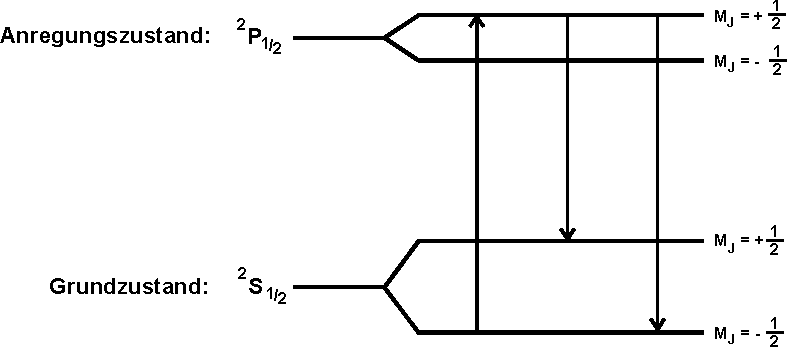
\includegraphics[width=0.7\textwidth]{Abb7.pdf}
	\caption[Optisches Pumpen]{Übergänge zwischen den Energieniveaus eines Alkali-Hüllenelektrons beim optischen Pumpen \cite{\V}}
	\label{fig:optischespumpen}
\end{figure}


